\chapter[Development of methodologies to complement metagenomic sequencing in an integrative study of Ace Lake]{Development of methodologies to complement metagenomic sequencing in an integrative study of  Ace Lake}
\label{ch:ace}
\acresetall

%-----------------------------------------------------------------------------------------------
\section*{Co-authorship statement}
\addcontentsline{toc}{section}{Co-authorship statement}

Sections from this chapter have been published as:\\

Federico M. Lauro, Matthew Z. DeMaere, \textbf{Sheree Yau}, Mark V. Brown, Charmaine Ng,
David Wilkins, Mark J. Raftery, John A.E. Gibson, Cynthia Andrews-Pfannkoch, Matthew Lewis,
Jeffery M. Hoffman, Torsten Thomas, and Ricardo Cavicchioli. 
An integrative study of a meromictic lake ecosystem in Antarctica. \emph{\underline{The ISME Journal}} 
5:879--895, 2011.

I performed the metaproteomic mass spectral analysis, epifluorescence microscopy imaging,
microbial and viral counts and wrote the corresponding sections of the publication.

Contributions by others that support the work presented in this chapter are as follows.
Research was designed by Federico Lauro, Mark Brown, Torsten Thomas, John Gibson and Ricardo Cavicchioli.
Sample collection was performed by Federico Lauro, Mark Brown, Torsten Thomas, Jeffery Hoffman and Ricardo Cavicchioli.
\textsc{DNA} extraction and clone library preparation was performed by Cynthia Andrews-Pfannkoch and Jeffery Hoffman.
\textsc{DNA} sequencing quality control was performed by Matthew Lewis.
Metagenomic sequence filtering, mosaic assembly and annotation was performed by Matthew DeMaere.
Protein extraction, one-dimensional sodium dodecyl sulphate-polyacrylamide gel electrophoresis and liquid chromatography mass spectrometry performed by Charmaine Ng.
Assistance in mass spectrometry was provided by Mark Raftery.
\newpage

%----------------------------------------------------------------------------------------------
\section{Abstract}
Ace Lake is a saline meromictic lake that is the most studied lake in the Vestfold Hills, Antarctica.
As a system of moderate biological complexity with extensive historic physical and chemical data, it was chosen as a site to implement an integrative study of the whole lake ecosystem.
Metagenomic analysis of Ace Lake revealed microbial taxa and metabolic genes were stratified according to the lake's water column structure and also was able to infer potential for nutrient cycling.
The aerobic mixolimnion resembles a marine surface water microbial community, the oxic--anoxic interface contains a near-clonal population of \ac{GSB} while the anoxic monimolimnion contains an extremely diverse assemblage that includes methanogenic \emph{Archaea} and \ac{SRB}.
The viral population comprises abundant bacteriophages as well as large phycodnaviruses that were detected at all depths of the lake, except for the \ac{GSB} layer \cite{Lauro2011}.

This study aimed to generate independent datasets complementary to metagenomic sequencing as part of the integrative analysis of the lake.
A method for visualising and enumerating cells and \acp{VLP} using epifluorescence microscopy was developed that does not require use of the relatively expensive Anodisc filters.
Microscopic examination confirmed that the sequential filtration procedure used to size fractionate the lake microbiota was effective. 
Furthermore, it determined the densities of cells and \acp{VLP} and independently verified the absence of \acp{VLP} associated with the lake's \ac{GSB}.

Preliminary metaproteomic analysis of the Ace Lake depth profile using cross-species matching of mass spectra to the \ac{NR} yeilded few protein identifications \cite{Ng2010b}.
However, metaproteomic analysis of the \ac{GSB} layer using matching \ac{GSB} metagenomic sequences as the search database gave a 3-fold increase in protein identifications and allowed detailled description of the metabolism of the \ac{GSB} \cite{Ng2010a,Ng2010b}.
By similarly using metagenomes matched to the metaproteome samples as search databases, significant improvements in protein identifications were made.
Application of the software package \textsc{Scaffold} to protein mass spectral analysis further improved validity of protein identifications and allowed for approximations of protein abundance using spectral counts.
These data were provided crucial to support a comprehensive description of the  entire Ace Lake ecosystem function. 

%---------------------------------------------------------------------------------------------
\section{Introduction}
\acresetall
Ace Lake is a meromictic saline lake in the Vestfold Hills that separated from the sea $\sim$5,000 BP \cite{Bird1991}. 
Extensive physical, chemical and biological data has been collected from Ace Lake in the last decades \cite{Rankin1999}.
%This is summarised in the figure of the whole lake. %figure of lake.
The system is microbially-dominated and of reduced diversity \cite{Bowman2000a} with the only metazoan life present being callanoid copepods. %Look up.
%What else? about the diversity from Bowman paper? Link to the intro.
Ace Lake is a highly stratified lake system that is 25 m at its deepest point.
It is ice-covered for $\sim$11 months of the year and generally thaws in January \cite{Rankin1999}.
Water is marine-derived and a largely neutral water balance has ensured salinity is close to that of seawater.
The lake is physically separated into an aerobic mixolimnion, a steep chemo/oxycline at 12.7 m and an anoxic monimolimnion.
The monimolimnion is sulfidic and methanogenic; both compounds have presumably accumulated through activity from \ac{SRB} and methanogenic archaea respectively \cite{Rankin1999, Lauro2011}.

As a physically and chemically well-characterised system of moderate diversity, Ace Lake was chosen as a model ecosystem to implement a whole systems level analysis to piece together ecosystem functioning.
Samples were obtained from the mixolimnion (5 and 11.5 m), the chemo/oxycline (12.7 m) and the monimolimnion (14, 18 and 23 m ).
Sampling was conducted as part of the \ac{GOS} expedition \cite{Rusch2007} by using size fractionation of microbial biomass onto 3.0, 0.8 and 0.1 \textmu{}m membrane filters.
Both metagenomic and metaproteomic analysis was conducted on these samples to assess the taxonomic composition, the metabolic potential and identify the active members of the community.

From the metagenomic analysis significant differences were found in taxonomic composition between each size fraction and between the three zones of Ace Lake \cite{Lauro2011}.
The clear difference between the size fractions indicated the sequential filtration process is an effective means to separate the community and that different sized populations in the community have different ecological roles (\emph{e.g.} particle attached copiotrophs or planktonic oligotrophs).
The mixolimnion community is similar to a marine surface water assemblage consisting of a high abundance of the SAR11 clade of \emph{Alphaproteobacteria} related to ``\emph{Candidatus} Pelagibacter ubique'' and green algae of the order \emph{Mamiellales}.
However, diversity is reduced by one order of magnitude \cite{Lauro2011}.
Unlike Southern Ocean surface water, the mixolimnion is overrepresented in \emph{Cyanobacteria} related to \emph{Synechococcus} and \emph{Actinobacteria}, which may represent taxa that mark the transition from a marine to lake community.
A dense, near-clonal population of \acl{GSB} related to \emph{Chlorobium} termed \emph{C}-ace reside at the chemo/oxycline at 12.7 m \cite{Ng2010a, Lauro2011}.
Below, in the monimolimnion is a diverse, primarily heterotrophic community with abundant \ac{SRB} and methanogenic \emph{Archaea}.
The viral community comprises \emph{Phycodnaviridae}, \emph{Myoviridae}, \emph{Siphoviridae}, \emph{Podoviridae} and unidentified viral families \cite{Lauro2011}. 
Bacteriophage sequences were abundant in the bottom waters, whereas the surface community, was dominated by phycodnaviruses \cite{Lauro2011}. 
Most notably, no viral signatures were found associated with the \ac{GSB} at the chemo/oxycline. 
Mathematical modeling predicted that the absence of bacteriophage predation in the \ac{GSB} could be due to an adaptation to longer cycles of growth and inactivity in response to the polar light regime \cite{Lauro2011}. 
%Phototrophs with faster growth rates, such as eucaryal algae and \emph{Cyanobacteria} in the surface water, were predicted to be more susceptible to viral predation \cite{Lauro2011}. 

Preliminary metaproteomic analysis along the vertical profile of Ace Lake has been performed using a cross species genomic database comprising the \ac{NCBI} \ac{NR} to perform protein identifications \cite{Ng2010b}.
A focused metaproteogeonomic analysis conducted on the dense \ac{GSB} layer using the matched \ac{GSB} metagenome as the database resulted in 3-fold increase in protein identifications compared to using the \ac{NR} database \cite{Ng2010b}.
%Put in a table of the rates of matches...
This indicates large gains in metaproteome coverage are possible using a matched metagenomic database \cite{Ng2010b}.
Significantly, \ac{GSB} appeared to be crucial in the lake ecosystem as they had the greatest genetic potential for nitrogen and carbon fixation as well as sulphur cycling \cite{Ng2010b, Lauro2011}.
Metaproteomic analysis was able to identify which proteins were actively expressed and thus the active pathways of the \ac{GSB} metabolism which are crucial to the function of the lake \cite{Ng2010a}.

This study aimed to develop and apply methodologies which provide independant data to complement an integrative metagenomic analysis of the whole Ace Lake ecosystem.
These included a modified epifluorescence microscopy procedure to determine cellular and viral densities and validate the efficacy of size-fractionation and a metaproteomic analysis workflow to identify proteins and estimate their abundance.

%---------------------------------------------------------------------------------------------

\section{Materials and methods}
\label{sec:ace_mm}
\subsection{Ace Lake samples}
Water samples were collected from Ace Lake (68$^{\circ}$28$'$23.2$''$S, 78$^{\circ}$11$'$20.8$''$E), Vestfold Hills, Antarctica on 21 and 22 December 2006. 
A 2 m hole positioned above the deepest point (25 m depth) of the lake was drilled through the ice cover of Ace Lake to reach the lake surface.
A volume of 1--10 L was collected by sequential size fractionation through a 20 \textmu{}m pre-filter directly onto 3.0, 0.8 and 0.1 \textmu{}m pore-size 293 mm polyethersulfone membrane filters \cite{Rusch2007}, along the depth profile.
Two independent sets of filters were obtained, one set for metagenomics and one for metaproteomics.
Filteres were placed into sterile 50 ml tubes containing a solution of 2.5 mM EGTA, 2.5 mM EDTA, 0.1 mM Tris-EDTA (pH 8), 1mM PMSF (freshly prepared), 50 \textmu{}l protease inhibitor cocktail VI (Calbiochem, San Diego, \textsc{CA}, \textsc{USA}) and the tubes placed in liquid nitrogen before storage at $-$80$^{\circ}$C.
The protease inhibitor cocktail has a broad specificity for inhibition of serine, cysteine, aspartic and metalloproteases within protein extracts.
Samples were taken in the order, 23, 18, 14, 12.7, 5 and finally, 11.5 m.

After samples from each depth were collected, the sample racks were sequentially washed with 2 $\times$ 25 L 0.1 N NaOH, 2 $\times$ 25 L 0.053\% NaOCl, and 2 $\times$ 25 L fresh water. 
The sample hose was flushed with water from each depth before being applied to the filters. 
A \emph{Chlorobium} signature was identified at 5 m, but not immediately above the \ac{GSB} layer at 11.5 m. 
As the next sample taken after sampling at 12.7 m was at 5 m, and then 11.5 m, despite all equipment being thoroughly washed with bleach, NaOH and water, 
the simplest explanation for the \ac{GSB} signature at 5 m is carry-over from sampling of the dense biomass at 12.7 m. 

A sonde probe (\textsc{YSI} model 6600, \textsc{YSI} Inc., Yellow Springs, \textsc{OH}, \textsc{USA}) was used to record depth, dissolved oxygen content, pH, salinity, temperature and turbidity throughout the water column of the lake. 
Total organic carbon was determined using a total organic carbon analyzer, TOC-5000A (Shimadzu, Kyoto, Japan) equipped with a \textsc{ASI}-5000A auto sampler (Shimadzu), and particulate organic carbon by standard protocols 
\url{(http://www.epa.gov/glnpo/lmmb/methods/about.html)} 
at the Centre for Water and Waste Technology, \textsc{UNSW}.

\subsection{\textsc{DNA} extraction, sequencing and data cleanup}
\textsc{DNA} extraction and Sanger sequencing was performed on 3730xl capillary sequencers (Applied Biosystems, Carlsbad, \textsc{CA}, \textsc{USA}) and pyrosequencing on \textsc{GS20 FLX} Titanium (Roche, Branford, \textsc{CT}, \textsc{USA}) at the \acl{JCVI} in Rockville, \textsc{MD}, \textsc{USA} \cite{Rusch2007}. 
The scaffolds and annotations will be available via \ac{CAMERA} and public sequence repositories such as the \ac{NCBI} and the reads will be available via the \ac{NCBI} Trace Archive. 

Sanger reads were trimmed according to quality clear ranges.
The quality of pyrosequencing reads was assessed as follows: 
a \ac{BLAST} nucleotide database was created from the Sanger reads of the 0.1 \textmu{}m fraction of samples GS230, GS231 and GS232 (see \tabreft{tab:ace_metag} for summary of the metagenomic data and sample IDs).
\begin{table}
\footnotesize
\caption[Summary of metagenomic data for Ace Lake profile]{Summary of metagenomic data for Ace Lake December 2006 profile. S, Sanger sequencing data; *scaffolds that were assembled from a hybrid of Sanger and 454 sequences.}
\label{tab:ace_metag}
\smallskip
\begin{tabularx}{\textwidth}{p{0.6cm}p{0.7cm}p{0.5cm}p{1.8cm}p{1cm}Xp{2.4cm}p{1.4cm}}
\toprule
\textbf{ID} & \textbf{Depth} & \textbf{Size}         & \textbf{Trimmed}      & \textbf{\acp{ORF}} & \textbf{Annotated}            & \textbf{$>$10 kbp} & \textbf{Annotated} \\
            & \textbf{(m)}   & \textbf{(\textmu{}m)} & \textbf{reads}        & \textbf{(reads)}   & \textbf{\acs{COG}/\acs{KEGG}} & \textbf{scaffolds} & \textbf{scaffold} \\
            &                &                       &                       &                    & \textbf{\acp{ORF}}            & \textbf{(reads)}   & \textbf{\acp{ORF}} \\
\midrule
GS232 & 5    & 0.1 & S: 281,490 & 421,252 & 112,490/96,771   & *               & *      \\
      &      &     & 454: 539,536    & 638,757 & 109,551/103,201  & 2,809 (349,015) & 45,281 \\
      &      & 0.8 & 454: 468,122    & 485,021 & 150,660/135,451  & 269 (66,743)    & 3,215  \\
      &      & 3.0 & 454: 160,835    & 138,191 & 24,920/22,240    & 33 (2,980)      & 353    \\ 
GS231 & 11.5 & 0.1 & S: 283,663 & 427,889 & 124,332/107,523  & *               & *      \\
      &      &     & 454: 523,650    & 608,671 & 99,175/95,266    & 2,814 (390,490) & 47,987 \\
      &      & 0.8 & 454: 474,419    & 511,909 & 218,126/176,332  & 174 (161,891)   & 2,321  \\
      &      & 3.0 & 454: 373,226    & 307,850 & 57,961/51,915    & 64 (8,139)      & 766    \\ 
GS230 & 12.7 & 0.1 & S: 54,446  & 75,576  & 42,790/41,391    & *               & *      \\
      &      &     & 454: 442,389    & 492,995 & 201,203/227,726  & 88 (282,232)    & 3,039  \\
      &      & 0.8 & 454: 529,711    & 555,328 & 209,078/234,682  & 86 (313,550)    & 2,187  \\
      &      & 3.0 & 454: 208,272    & 215,741 & 80,925/77,340    & 75 (49,942)     & 1,792  \\ 
GS229 & 14   & 0.1 & S: 10,042   & 14,326  & 5,261/4,469      & *               & *      \\
      &      &     & 454: 413,992    & 458,942 & 100,045/88,300   & 228 (22,556)    & 2,443  \\
      &      & 0.8 & 454: 453,205    & 435,534 & 142,743/129,403  & 139 (45,083)    & 2,118  \\
      &      & 3.0 & 454: 291,065    & 301,580 & 105,756/89,188   & 31 (2,422)      & 262    \\ 
GS228 & 18   & 0.1 & S: 9,672    & 15,077  & 3,667/3,008      & *               & *      \\
      &      &     & 454: 362,490    & 389,077 & 51,312/44,290    & 29 (1,815)      & 260    \\
      &      & 0.8 & 454: 544,302    & 556,243 & 186,455/163,878  & 154 (14,806)    & 1,334  \\
      &      & 3.0 & 454: 278,846    & 287,423 & 95,876/81,161    & 2 (131)         & 15     \\ 
GS227 & 23   & 0.1 & S: 100,085 & 160,302 & 33,462/27,302    & *               & *      \\
      &      &     & 454: 482,527    & 547,170 & 84,257/73,074    & 1,136 (51,163)  & 12,339 \\
      &      & 0.8 & 454: 553,234    & 611,717 & 161,973/137,632  & 105 (7,904)     & 825    \\
      &      & 3.0 & 454: 264,160    & 270,188 & 85,596/72,206    & 6 (287)         & 48     \\ 
TOTAL &      & -   & 8,103,379       & 8,926,759 & 2,487,574/2,283,749 & 8,269 (1,771,149) & 126,585 \\ 
\bottomrule
\end{tabularx}
\end{table}

After performing a \ac{BLAST} comparison of the corresponding pyrosequencing reads against each Sanger sequence database with a minimum bitscore of 80 and maximum e-value of 0.1, reads were binned according to length.
The percentage of reads for each bin lacking a match to the Sanger read database was recorded. 
The percentage reads at least 25\% repetitive after \textsc{MDUST} \cite{Morgulis2006} analysis at default settings, and the percentage of reads containing N's, were assessed. 
In contrast to earlier pyrosequencers \cite{Huse2007}, no length-dependent bias in reads containing N's was observed. 
However, short reads had a disproportionately high number of repeats. 
Moreover, based on the proportion of reads with no match to the Sanger data set, both very short and very long reads had a disproportionately high number of errors; an observation that was previously reported \cite{Huse2007}.

On the basis of this analysis, a three step filtering process was applied to each sample. 
Reads were initially run through the Celera \textsc{sffToCA} \cite{Miller2008} pre-processor followed by \textsc{Lucy} \cite{Chou2001} and finally, excluding the bottom 8\% and top 3\% of reads determined from the read length distribution. 
As the \textsc{sffToCA} (v5.3) pre-processor removes all reads with a perfect prefix of any other read it overcomes the `perfect duplicates' problem \cite{Gomez-Alvarez2009}.
 
After this process, $<$5\% of the reads belonged to clusters of duplicates with three or more reads, and \ac{COG} of proteins classification of these reads showed an over-representation of category L (replication, recombination and repair) that includes mobile genetic elements, which are often duplicated, suggesting a potential biological significance for the duplicated reads. 
It is possible these residual duplications are a result of high gene copy number or localized fragility of DNA sequences that might be biasing the shear points.

\subsection{Metagenomic DNA assembly and annotation}
Mosaic assemblies were generated for each sample fraction using Celera \ac{WGS} Assembler v5.3 \cite{Myers2000}. 
For each assembly, the runtime parameters used were as outlined for 454 sequencing data in the published standard operating procedure\\ 
\url{(http://sourceforge.net/apps/mediawiki/wgs-assembler/index.php?title 1⁄4SFF\_SOP)}. 
As none of the samples can be considered clonal, these are regarded as stringent assemblies \cite{Rusch2007}. 
Each 0.1 \textmu{}m fraction assembly was a hybrid of Sanger and 454 read data, wherein the estimated genome size was manually set to minimize the number of unitigs from abundant organisms being falsely classified as degenerate \cite{Rusch2007}. 
Annotation of each sample fraction assembly was carried out using an in-house pipeline, wherein the pipeline stages consisted of genomic feature detection and subsequent annotation \cite{DeMaere2011}. 
Detected features consisted of \acp{ORF}, transfer \textsc{RNA} and \ac{rRNA}. 
Each detected \ac{ORF} was further annotated by \ac{BLAST} comparison against \ac{NR}, Swissprot and \ac{KEGG}-peptide sequence databases and by \ac{HMMER} comparison against \ac{TIGRFAM} \cite{Haft2001}, \ac{COG} \cite{Tatusov1997, Tatusov2003} and known marker genes \cite{vonMering2007}.
In all cases the cut-off e-value was a maximum of 1e$-$5. 


\subsection{Epifluorescence microscopy}
Samples of unfiltered lake water and the flow-through from 3.0 and 0.8 \textmu{}m filters from all depths were collected on November 2008 and fixed on site in formalin 1\% (v/v). 
The samples were stored at $-$80$^{\circ}$C for subsequent direct counts of cells and \acp{VLP}. 
Enumeration was performed according to the method of \citet{Patel2007} with modifications. 
Lake water samples were filtered onto 0.01 \textmu{}m pore-size polycarbonate filters (25 mm Poretics, \textsc{GE} Osmonics, Minnetonka, \textsc{MN}, \textsc{USA}). 
Filters were air dried, then placed with the back of the filter on top of a 30 ml aliquot of 0.1\% (w/v) molten low-gelling-point agarose and allowed to dry at 30$^{\circ}$C. 
Samples were stained by the addition of 2 \textmu{}l working solution (1 in 400 dilution in 0.02 \textmu{}m filtered sterile Milli-Q) of \textsc{SYBR} Gold$^{\textregistered}$ (Molecular Probes, Eugene, \textsc{OR}, \textsc{USA}) to 20 \textmu{}l of mounting medium (\textsc{VECTASHIELD} HardSet, Vector Laboratories, Burlingame, \textsc{CA}, \textsc{USA}). 
Stained samples were counted immediately.
Samples were visualised under wide-blue filter set (excitation 460--495 nm, emission 510--550 nm) with an epifluorescence microscope (Olympus BX61, Hamburg, Germany).


\subsection{Protein extraction}
Proteins were extracted from membrane filters from all 0.1 \textmu{}m fractions from the six depths (5, 11.5, 12.7, 14, 18 and 23 m) according to the protocol developed by \citet{Ng2010a}, which is as follows.
The 0.1 \textmu{}m filters were allowed to thaw at room temperature and cut into quarters asceptically.
Separate extractions were performed on each filter quarter which served as technical replicates.
Each quarter filter was suspended in a lysis buffer containing 10mM Tris-EDTA (pH 8)(Univar), 20 \textmu{}l of protease inhibitor cocktail VI (Calbiochem), 0.1\% sodium dodecyl sulphate (Univar), and 1 mM dithiothreitol (Sigma-Aldrich).
Three freeze-thaw cycles were performed using liquid nitrogen.
The membrane was then removed, and the buffer was subject to five cycles of sonication of 40 s on a 30 \% duty cycle at power setting of 3, which serves to lyse any remaining cells and shear nucleic acids.
The mixture was centrifuged at 5000 \emph{g} for 25 min at 4$^{\circ}$C to remove insoluble material.
Smaller insoluble particles were removed by filtration through a 0.22 \textmu{}m syringe filter (Millipore).
Buffer exchange with 30 ml of 10 mM Tris-EDTA (pH 8) and concentration of soluble extracted proteins was performed in a 5 kDa cut-off Amicon Ultra-15 filter unit (Millipore).
Protein concentration was determined using a bicinchoninic acid protein assay kit (Sigma-Aldrich).

\subsection{Metaproteome \acs{1D-SDS-PAGE} and \acs{LC}-\acs{MS-MS}}
Extracted proteins were separated by \% \ac{1D-SDS-PAGE} containing 12 \% SDS using a Mini-PROTEAN system (Bio-Rad) as described previously \cite{Saunders2006}.
Trypsin digestion, \ac{LC} and mass spectrometry was conducted according to \citet{Ng2010a} as follows.
The gels were silver stained and the images of the resulting gel acquired with a UMAX PowerLook 1000 flat-bed scanner (Fujifilm).
Each lane containing the size separated proteins were excised and sliced according to size with a sterile scalpel.
Gel slices were washed in sterile Milli-Q water followed by acetonitrile, then subject to a series of reductioin, alkylation and dehydration reactions.
Digestion of proteins with trypsin was conducted by rehydrating gel pieces in a buffer of 200 ng trypsin (Promega) and 10 mM NH$_4$HCO$_3$ at 37$^{\circ}$C overnight. 
Gel slices were dehydrated in acetonitrile in a centrifugal evaporator (SpeedVac).

Peptides were rehydrated in 1 \% formic acid and 0.05 \% heptafluorobutyric acid and separated by nano \ac{LC} using an Ultimate 3000 \acs{HPLC} and autosampler system (Dionex).
Samples of 2.5 \textmu{}l were concentrated and desalted onto a micro C18 precolumn (500 \textmu{}m $\times$ 2 mm; Michrom Bioresources) with H$_2$O:CH$_3$CN (98:2, water to 0.05\% heptafluorobutyric acid) at 20 \textmu{}l min$^{-1}$.
After a 4 min wash, the precolumn was switched into line (Valco 10 port valve; Dionex) with a fritless nano column (75 \textmu{}m $\times$ 10 cm) containing C18 medium (5 \textmu{}, 200 \AA Magic, Michrom).
Peptides were eluted using a linear gradient of H$_2$O:CH$_3$CN (98:2, 0.1\% formic acid) to H$_2$O:CH$_3$CN (63:36, 0.1\% formic acid) at 350 nl min$^{-1}$ over 30 min.

1800 V was applied to the low volume tee (Upchurch Scientific) and the column tip was positioned $\sim$0.5 cm from the heated capillary (250$^{\circ}$C of an LTQ-FT Ultra mass spectrometer (Thermo Electron).
Positive ions were generated by electrospray and the LTQ-FT Ultra was operated in data-dependent acquisition mode.
A survey scan \emph{m/z} 350--1,750 was acquired in the FT ICR cell (resolution $=$ 1,000,000 ions in the linear ion trap).
Up to the six most abundant ions ($>$3,000 counts) with charge states of $+$2, $+$3 or $+$4 were sequentially isolated and fragmented within the linear ion trap using collision-induced dissociation with an activation $q$ $=$ 0.25 and activation time of 30 ms at a target mass value of 30,000 ions.
\emph{m/z} ratios selected for \ac{MS-MS} were dynamically excluded for 30 s.
Peak lists were generated using \textsc{extract\_msm} from \textsc{Mascot Daemon} (Matrix Science, Thermo) using the default parameters.

\subsection{Mass spectra analysis and validation of metaproteomic identifications}
The specta generated from \ac{MS} were searched against the protein sequence database corresponding to that depth constructed from the 0.1 \textmu{}m mosaic assemblies using \textsc{Mascot} (Matrix Science).
\textsc{Mascot Distiller} (Applied Biosystems) was used as the data import filter with the following criteria applied to the \ac{MS-MS} ion search: a maximum of one missed cleavage for trypsin, peptide mass tolerance of $\pm$ 4 ppm, a fragment mass tolerance of $\pm$0.6 Da and variable modifications of acrylamide, carbamidomethyl and oxidation.
The number of protein sequences in each database were as follows: 5 m, 138,208; 11.5 m, 133,948; 12.7 m, 27,142; 14 m, 62,436; 18 m, 71,512; and 23 m, 128,878. 
\textsc{Scaffold} (version Scaffold\_2\_05\_01, Proteome Software Inc., Portland, \textsc{OR}, \textsc{USA}) was used to validate \ac{MS-MS}-based peptide and protein identifications. 
Peptide and protein identifications were accepted if they could be established at $>$95\% and 99\% probability, respectively, as specified by the \textsc{Peptide Prophet} algorithm \cite{Keller2002}. 
Protein identifications required the identification of at least two peptides.
 
Proteins that contained similar peptides and could not be differentiated based on \ac{MS-MS} analysis alone were grouped to satisfy the principles of parsimony and are referred to as a protein group. 
Spectral counting was used to semi-quantitively estimate protein abundance. 
The total assigned spectra that matched to each identified protein were exported from \textsc{Scaffold} 2.0. 
For similar proteins that have shared peptides (a protein ambiguity group), spectra were assigned to the protein with the most unique spectra. 
To normalise for variation in total spectra acquired between sample replicates, the number of spectra of each protein was multiplied by the average total spectra divided by the total spectra of the individual replicate. 
The spectral count of each protein was averaged across the replicates. 
As longer proteins are more likely to be detected, the average spectral counts were divided by the length of the protein. 
This value is equivalent to the normalised spectral abundance factor \cite{Florens2006, Zybailov2006}. 
In order to compare the relative abundance of proteins between depths, the normalised spectral abundance factor was divided by the average read depth of the contig (scaffold or degenerate) to which the protein mapped. 

If $>$90\% of a scaffold’s length consisted of surrogate (highly degenerate unitig) sequence, the average read depth of the surrogate was used. 
For identified proteins that were part of a protein group the longest protein length and largest read depth value in the group was used. 
Pairwise comparisons of each zone were conducted on \ac{COG} assigned proteins. 
The normalised spectral counts from each protein was aggregated based on their \ac{COG} annotation. 
All proteins that were part of an ambiguity group were confirmed to share the same \ac{COG} annotation to ensure counts were not biased because of the common spectra.

The summed spectral counts from 5 and 11.5 m (mixolimnion), and 14, 18 and 23 m (monimolimnion) were pooled. 
Statistical significance of differences between each zone was assessed using Fisher's exact test, with confidence intervals at 99\% significance calculated by the Newcombe–Wilson method and Holm-Bonferroni correction (P-value cutoff of 1e$-$5) in \ac{STAMP} \cite{Parks2010}. 
All proteins identified, including their gene identifier, normalised spectral abundance, \ac{COG} and \ac{KEGG} Orthology identifiers, \ac{KEGG} locus tag and matching \ac{COG} or \ac{KEGG} description are provided in Appendix Tables \tabreft{tab:ace_protids_5m}--\tabref{tab:ace_protids_23m}.



%---------------------------------------------------------------------------------------------

\section{Results and discussion}

\subsection[Epifluorescence microscopy methodology]{Development of epifluorescence microscopy methodology for cell and \acp{VLP} enumeration}
As part of the integrative study of Ace Lake, an epifluorescence microscopy methodology was developed.
There were several important outcomes expected from visualisation of microbiota from size fractionated water samples. 
Firstly, visualising microbiota from water samples allows examination of cellular morphologies and enumeration of cells and \acp{VLP}.
Absolute cellular and \ac{VLP} densities are not able to be inferred from the metagenomic data and necessitates an independent method of determination.
Determining viral densities is extremely important as the first studies to do so found that viruses are the most numerous biological entities on the planet and likely play a large role in plankton mortality in the ocean \cite{Bergh1989,Proctor1990}. %Why is determining cellular densities important
\ac{VLP} counts from marine environments vary with depth and trophic status ranging from 10$^6$ to 10$^8$ \acs{VLP} ml$^{-1}$ \cite{Suttle2005}. %cite Fuhrman review paper too.
Viral counts from various aquatic environments have differed from site to site indicating a variable role of virally mediated mortality. %ref microbial ecology of the oceans.%cite Fuhrman review.
Secondly, size fractionation of suspended microbial biomass from aquatic environments has been utilised as part of the landmark Sargasso Sea metagenomic study \cite{Venter2004} and subsequent \ac{GOS} expedition \cite{Rusch2007}.
The Ace Lake samples were collected using the same sampling strategy as the \ac{GOS} dataset but has sequence information from all three filter sizes. 
Thus, the visualisation of microbial morphologies from each stage of the filtration process would determine efficacy of the filtration process.

Developing a revised method for the simultaneous counts of cells and \acp{VLP} was necessary due to inability to source 25 mm diameter 0.02 \textmu{}m pore-size Anodisc filters (Whatman) that have been long used with fluorescent nucleic acid dyes for this purpose \cite{Hennes1995, Noble1998, Patel2007}. 
They were marked for discontinuation in December 2008 after the take over of Whatman by \textsc{GE} Healthcare and was the cause of a global shortage that was strongly opposed by the viral ecology community \cite{Torrice2009}.
Since conducting this research, production of 25 mm Anodisc filters has resumed, albeit at much greater cost per filter. 
The need to develop alternative methodolodies has been great enough that protocols were developed independently by research groups \cite{Budinoff2011, Diemer2012} stressing the utility of alternatives.

Clear \ac{PCTE} membrane filters were selected for use as a viable alternative product as they have defined pore-size of a sufficiently small diameter (0.015 \textmu{}m) required to capture \acp{VLP}. 
Furthermore, they have previously been used for \acp{VLP} enumeration \cite{Hara1991, Proctor1992} although using a different protocols, have a long history of use with cellular enumeration \cite{Hobbie1977} and therefore require no new materials to be easily adopted for use.
Finally, they are approximately 10$\times$ cheaper than the use of Anodiscs and are not subject to drops in availability.
However, \ac{PCTE} membranes have several reported shortcoming that have precluded their standard use for viral enumeration.
The 0.01 \textmu{}m 25 mm \ac{PCTE} filters are difficult to handle compared to 25 mm Anodisc filters that have a plastic support ring around the edge.
Also, \ac{PCTE} filters appear to have higher background fluorescence, have a slow flow rate taking $\sim$1--1.5 hours to filter 2 ml \cite{Hara1991} and have been reported to give \ac{VLP} counts an order of magnitude lower than that of Anodiscs \cite{Budinoff2011}.%more ref?

The protocol used is detailled in the materials and methods \ref{sec:ace_mm} where main challenges of using \ac{PCTE} were overcome for the purposes required for this study.
0.01 \textmu{}m pore-size \ac{PCTE} filters can form creases or wrinkles when mounted in the glass vacuum filter.
Good placement of the \ac{PCTE} filter was achieved by touching the edge of the \ac{PCTE} filter against the damp backing filter, making sure it was aligned and then gently and evenly releasing it in a single direction. 
0.01 \textmu{}m pore-size \ac{PCTE} filters also easily become statically charged and will become attracted to surfaces so careful handling is required during transport and manipulation. 
The greatest drawback in the use of \ac{PCTE} filters of such small pore-size is they similarly have a tendency to crinkle when mounted on the glass slide that can make visualisation of cells and \acp{VLP} on a single focal plane difficult.
Agarose was used to embed the filters to help flatten the membrane and aid in mounting.
However, this was not strictly necessary if filters are dried well, the membrane is mounted in the same way as as described for mounting on the vacuum filter and pressed flat against the glass slide with a minimal volume of mountant.
Even though careful handling is possible, this method likely requires more technical replicates that Anodisc filters because any \acp{VLP} outside the focal plane will not be counted.
Furthermore, as similarly reported by \citet{Diemer2012} for 0.03 \textmu{}m \ac{PCTE} membranes, distribution of \acp{VLP} on the membrane appears more variable than for Anodiscs with local regions devoid of \acp{VLP} and others with \acp{VLP} pooling.
The patchier \acp{VLP} distribution was attributed to greater irregularity in pores distribution compared to that of Anodisc filters and was considered to be the main contributing factor to variability in \ac{VLP} counts \cite{Diemer2012}

High back ground fluorescence was not observed when stain is only incorporated into the mountant after filtration rather than staining in the column before filtration.
This is one key difference between this protocol and others developed that use \ac{PCTE} membranes \citet{Hara1991, Proctor1992, Diemer2012}.
Other protocols have used 0.08 \textmu{}m membranes pre-stained with Irgalan Black \cite{Proctor1992} or 0.03 \textmu{}m pre-stained with Sudan black B \cite{Diemer2012} to minimise background fluorescence.
Filtration onto the \ac{PCTE} membranes with pore-size as small as this study was only found to be reported once \citet{Hara1991}.
Such a small pore-size necessitates a very strong seal of the filter column against the glass with absolutely no air leaks.
Leakage can be eliminated by sealing the fritted based to the column with laboratory film which ensures sample flow through the filter. 
However, the slow flow-rate was not a property of the \ac{PCTE} filters that could be overcome.
As the filtration and visualisation was performed on fixed samples in the laboratory rather than in the field, the time taken for filtration of 2--3 hours for each sample was not deemed problematic for the purposes of this study.
Counts of \acp{VLP} have been shown to decrease dramatically with time even when preserved with aldehyde-based fixatives \cite{Wen2004}.
Collecting larger sample volumes and flash freezing at $-$80$^{\circ}$C helps to slow this effect.
Due to logistic contraints with working in Antarctic environments, counts in the field were not possible so \acp{VLP} counts are expected to be underestimated.
However, all samples were processed within a similar time frame so the relative \acp{VLP} abundances down the depth profile and between size fractions are expected to be accurate as all samples would have undergone comparable amounts of \acp{VLP} loss. 

Overall, a viable alternative methodology was successfully developed for visualisation and enumeration of cells and \acp{VLP} using \ac{PCTE} membrane filters for use in this study \figref{fig:ace_microscopy}.
\begin{figure}
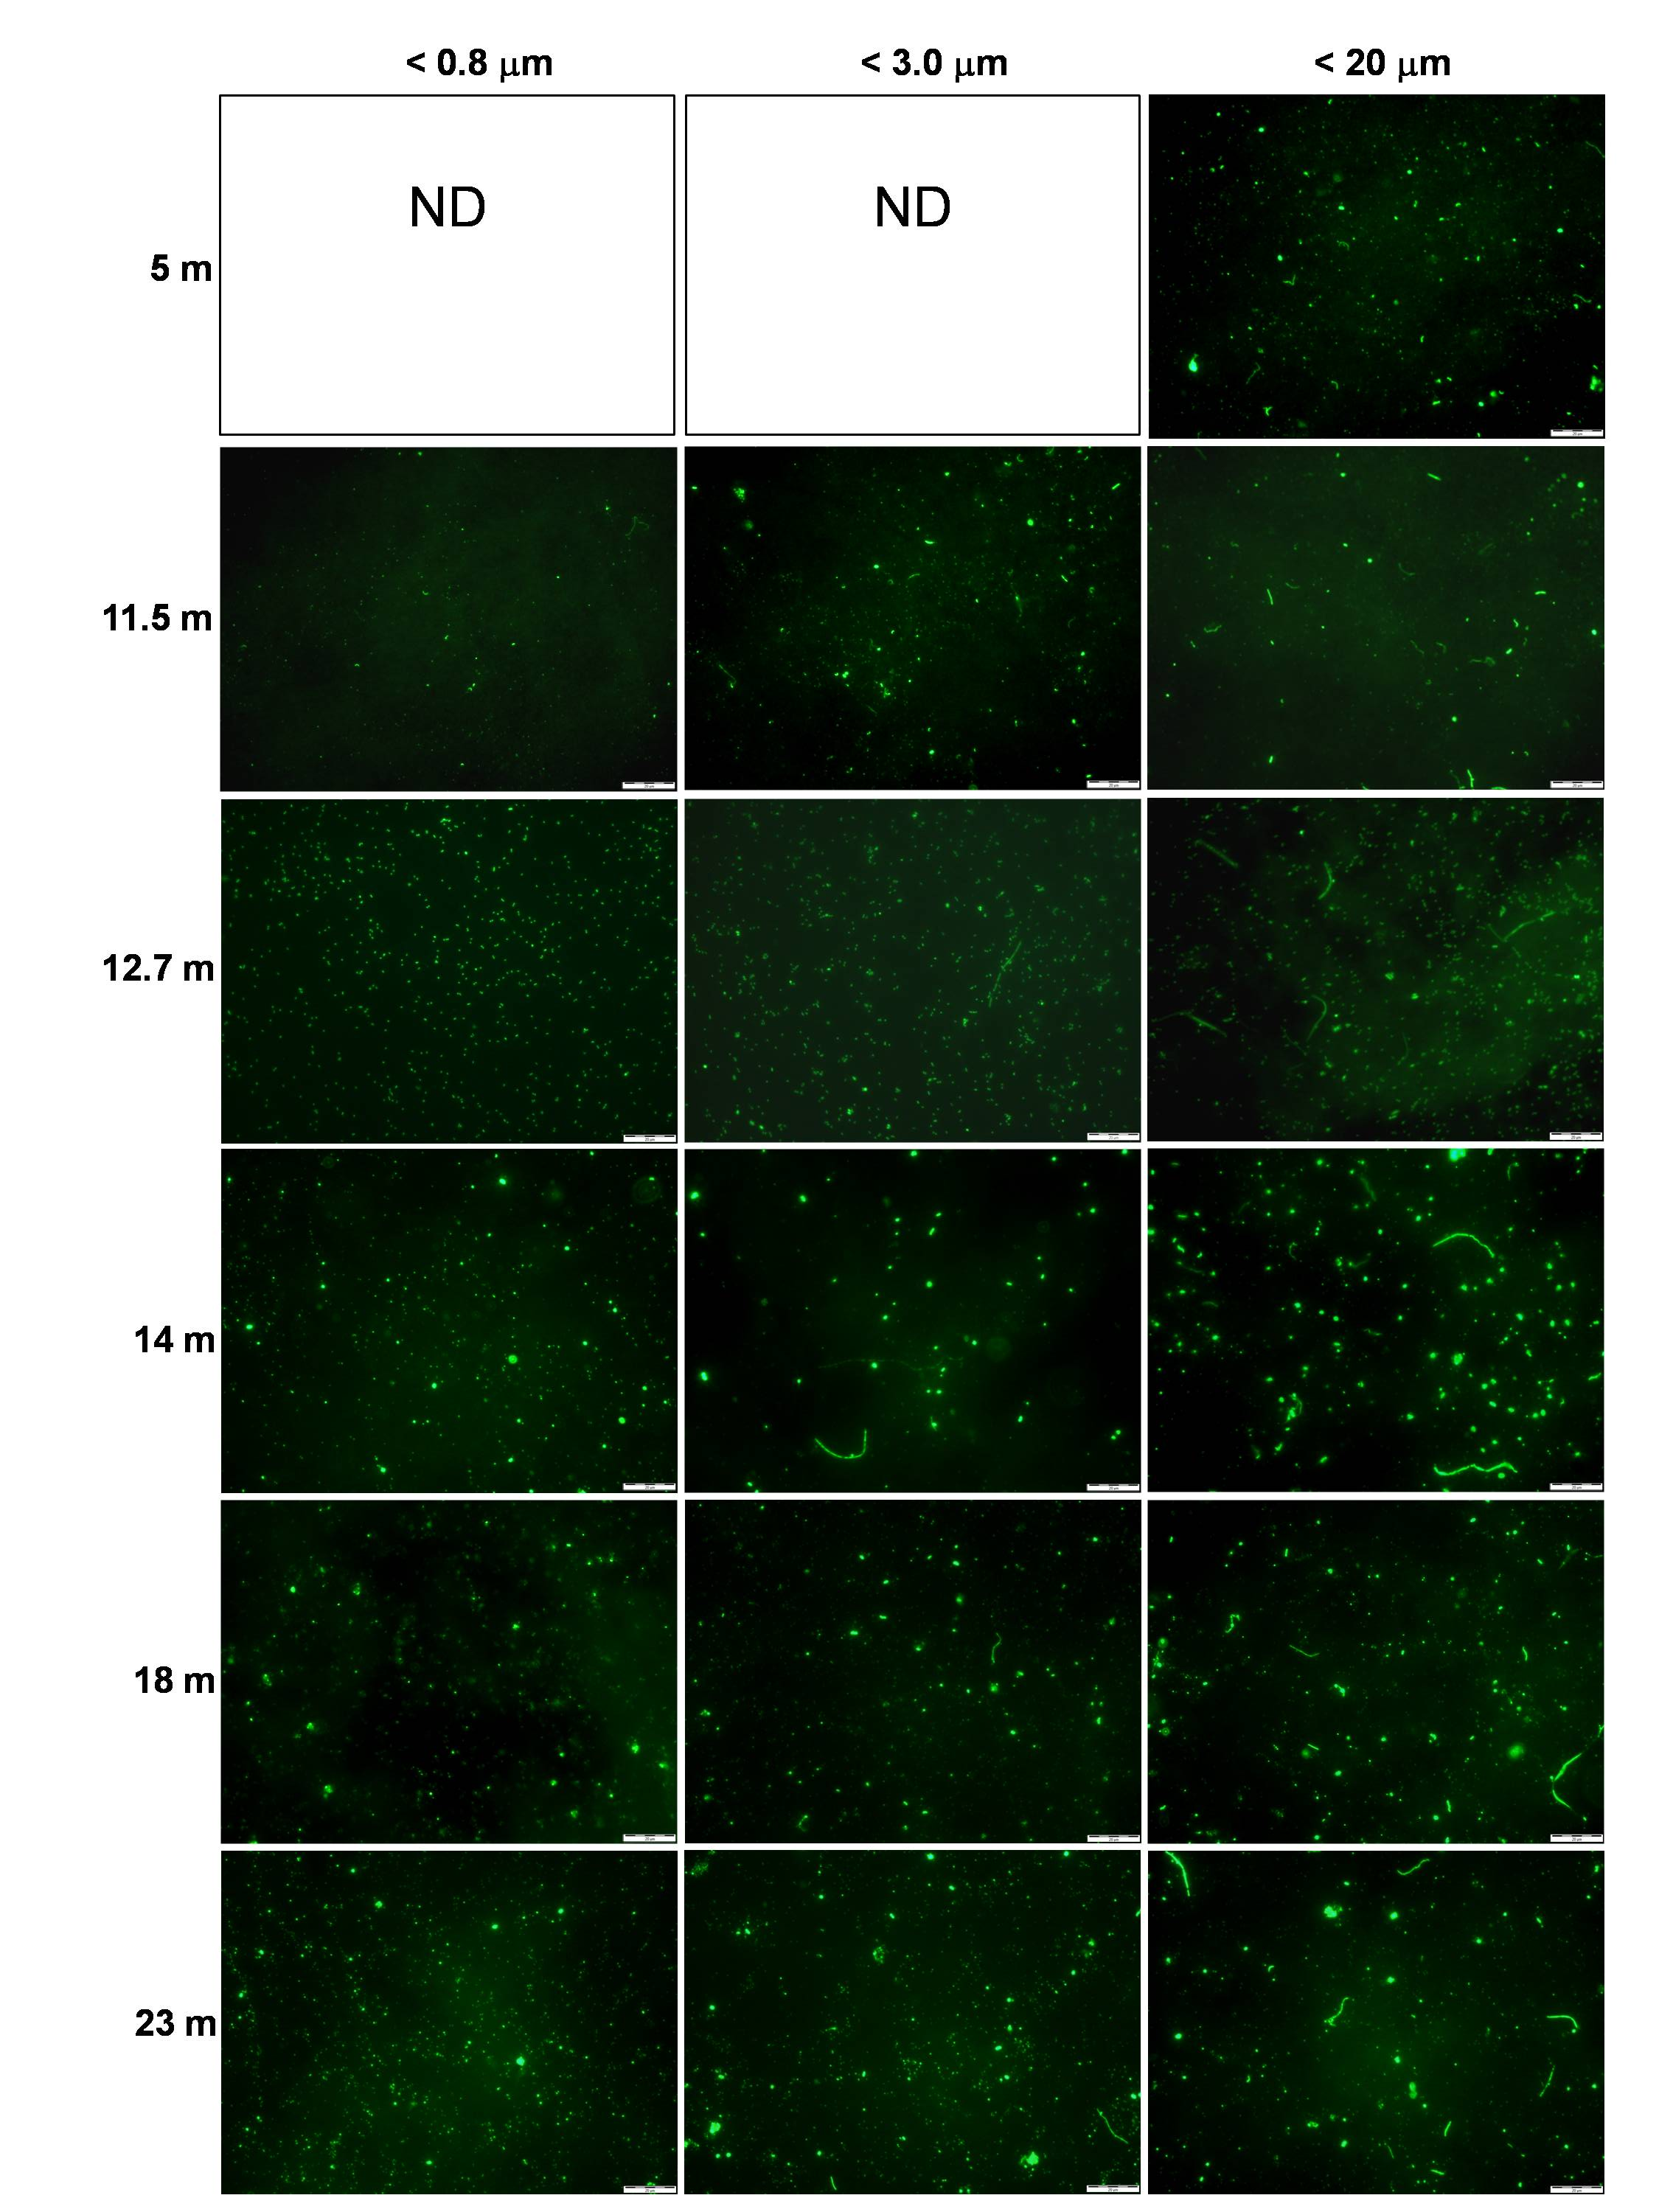
\includegraphics[width=\textwidth]{ace_figures/ace_microscopy.jpg}
\caption[Epifluorescence microscopy of Ace Lake microbiota]{Epifluorescence microscopy images of Ace Lake microbiota. Scale bar $=$ 20 \textmu{}m. ND, not determined.
}
\label{fig:ace_microscopy}

\end{figure}

To be a competitive alternative to Anodisc filters in terms of accuracy requires a further work that compares counts using this methodolody and the current standard Anodisc-based protocol \cite{Patel2007} with viral samples of known densities.

\subsection[Community stratification supported by cell and \ac{VLP} densities]{Size and depth stratification of the community supported by cell and \ac{VLP} densities}
Development of fluorescence microscopy methodology using 0.01 \textmu{}m pore-size polycarbonate filters for simultaneous cellular and viral counts shows:

1. Size fractionation procedure appeared effective.

2. Morphological differences supports stratification of the community.

3. Visualisation of the morphology supported the metagenomic data that saw size fractionated and taxonomically stratified community.

4. Virus to bacteria ratios can give important information about the community.

At 12.7m depth, the light levels, and the sharp transition in oxygen content and salinity (Fig. S2) favour the dominance of a very high-density (2.2 $\times$ 10$^8$ cells ml$^{-1}$) of a single type of \ac{GSB} of the genus \emph{Chlorobia}, refered to as C-Ace \cite{Ng2010a}. 
Viral signatures were essentially devoid in this zone. 
The ratio of bacteriophage to total viral population increased proportionally in the larger size fractions consistent with trophic analyses that indicate that the larger size fractions are mostly copiotrophic (Fig. S8) particle attached bacteria and therefore likely to be sensitive to lysogenic phage infection \cite{Lauro2009}. 
The 23 m unfiltered lake water contained very high levels (1.3 $\times$ 10$^8$ \acp{VLP} ml$^{-1}$) of \acp{VLP}. 
The high diversity of bacteria and archaea in all size fractions of the monimolimnion (Fig. 2) is consistent with the presence of a high viral population (Rodriguez-Valera et al., NRM, 2009).


%---------------------------------------------------------------------------------------------

\subsection[Development of methodology for protein identification of the metaproteome]{Development of methodology for protein identification of the metaproteome}

Identification of proteins from a biological sample (proteomics) indicates which portions of a genome are expressed under a set of given conditions.
This information is particularly relevant in microbial ecology as the presence of a gene does not necessarily mean it is functional but its identification of in the enviromental proteome (metaproteome) indicates an active microbial process.
However, the `shotgun' proteomics procedure using high sensitivity tandem mass spectrometry pioneered for use in metaproteomics \cite{Ram2005} presents significant methodological challenges.

A general shotgun proteomics workflow is shown in \figreft{fig:workflow}.
It shows that apart from successful sample preparation to simplify the complex protein mixture, successful protein identification depends greatly upon the genomic database, the search algorithm and criteria used to make the protein identification.
\begin{figure}
\centering
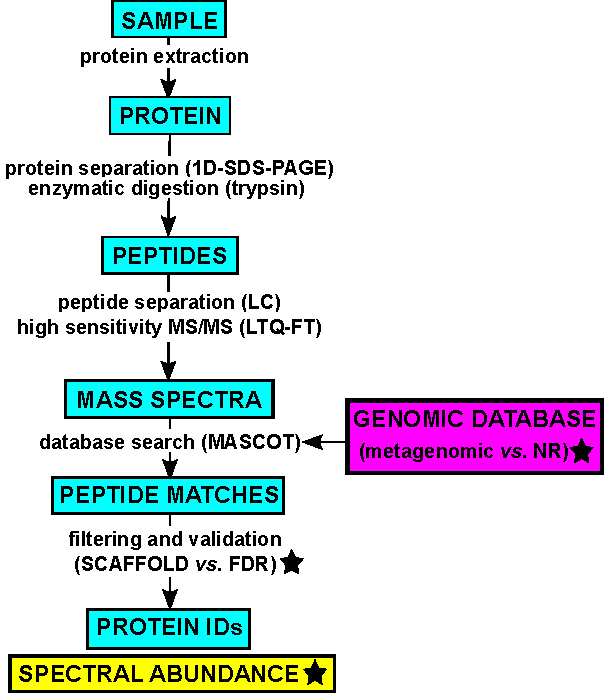
\includegraphics[width=80mm]{ace_figures/workflow.pdf}
\caption[General shotgun proteomics workflow]{A general shotgun proteomics workflow showing how proteins are identified. The procedures or materials used in this study are specified in parentheses. The steps in the workflow that were developed in this study are marked with a star.
}
\label{fig:workflow}

\end{figure}

This due to how the tandem mass spectra are used to identify proteins (see \citet{Marcotte2007} for a primer on shotgun proteomic identification).
Briefly, proteins are extracted from the sample and enzymatically digested to generate peptides.
The peptides are separated by \ac{LC} and subject to the first round of mass spectra acquisition where the mass of the peptides, the precursor ion spectra, are detected.
Selected peptides undergo collision-induced dissociation where they fragment preferentially at the peptide bond.
The second round of mass spectra is acquired of the peptide fragments, the fragment ion spectra, that represents to the amino acid sequence of the peptide.
An \emph{in silico} enzymatic igestion is performed on the coding sequences of the genomic database to predict the precursor ion masses and their corresponding fragment ion spectra.
The fragment ion spectrum and precursor ion mass is used to determine the most likely amino acid sequence of the peptide by comparison to the genomic database and infer the identity of the protein(s) of origin of the peptide.

The challenges presented by protein identification are as follows.
Firstly, since protein identification hinges on the quality of the search database, \emph{i.e.} availability of matching genomic sequences with sufficient coverage and to some extent, accurate \ac{ORF} prediction, can have a large effect on protein identification.
This problem is compounded in metaproteomics as matching metagenomic sequences are not always available so cross-species matching using related genomes must be performed instead.
The success of cross-species matching then varies with how related the protein sequences are as a single amino acid change is sufficient for a peptide to be not be matched.
Furthermore, even if a corresponding metagenome is available, complete coverage of all genomic information from an environment is unlikely from all but the most simple of systems so it is expected that the rate of spectra matching will be lower in a metaproteome.

Secondly, heterogeneity can cause ambiguity in protein identifications.


Preliminary metaproteomic Total protein from the 0.1 \textmu{}m size fraction filters were extracted.
1. Using a matched metagenome instead of \ac{NR} for protein identification greatly increased the number of identifications.
1.1 Except at the bottom zone, likely because the community is too diverse so greater coverage of the metagenome is required. %see available good spectra vs good reads
In parallel with taxonomic diversity increasing with depth (with the exception of the GSB layer), the rate of metaproteomic identification of proteins decreased with depth (Table S2). 
The majority of the proteins that were detected (e.g. 67\% at 23 m) were for hypothetical proteins that tended to lack orthologues in well-characterized organisms, highlighting both the functional importance and novelty of this anaerobic zone of the lake.


2. More specific information could be assigned to the taxonomic groups such as.
2.1. The Actinobacteria sequences in the mixolimnion were associated with a diverse phylogenetic cluster (Luna cluster) mainly contributed by freshwater ultramicrobacteria \cite{Hahn2003}. 
Several Luna cluster isolates contain rhodopsin genes \cite{Sharma2009} and similar gene sequences were present in the Ace Lake oxic zone data and found to be expressed (167820670 and 163154474; Table S2).
2.2.This is consistent with the identification of \ac{CRISPR} associated \ac{CAS} proteins Cse2, Cse3 and Cse4 (165526330, 165526332 and 165526334, respectively) in the 12.7 m metaproteome (Table S2). 
The \ac{CAS} gene locus (cas3, cse1, cse2, cse3, cse4, cas5, cas1b), to which the proteins map, shares its organisation with \ac{CAS} loci of sequenced \ac{GSB}, and groups with the \emph{E. coli} subtype/variant 2. The \ac{CRISPR}/\ac{CAS} system is likely to confer phage resistance to C-Ace, akin to the role in other organisms (Karginov and Hannon 2010; Horvath and Barrangou 2010).
%Recall that GSB all have large CRISPR regions and that the one in C-ace appears to be much reduced. Could this imply a lessening of viral load? The intervening spacers do not match to known viral sequences
% but did match to other GSB, could they be for competition?

3. Using \textsc{Scaffold} to validate protein identification and perform spectral counts was helpful. 
3.1Same protein identifications as Charmaine except one or two.
3.2 Able to quantify differences between mixolimnion and monimolimnion.
The diversity and abundance of \ac{ABC} transporters was lowest in the 0.1 \textmu{}m fractions at 23 m (Fig. 3), and a correspondingly low number were detected in the metaproteome (Table S2). 
In contrast, numerous transporters, predominately \ac{ABC} type, were identified in the metaproteome of the mixolimnion samples, with a high \ac{COG} representation of transporters for carbohydrates ($\sim$34\% of normalised spectra), amino acids ($\sim$32\%) and inorganic ions ($\sim$9\%) (Table S2 and Fig. S11).
All transporters in the metaproteome were of bacterial origin and conservative phylum level assignments of the normalised spectra showed the majority to originate from \emph{Proteobacteria} (69\%), 
of which SAR11 comprised 46\% and \emph{Actinobacteria} 19\% (Table S2). 
A high proportion of expressed genes with transport functions have also been reported for SAR11 from coastal (Poretsky et al. 2010) and open ocean waters (Sowell et al. 2009) (Morris et al. 2010?). 
Oligotrophs, such as SAR11 not only posses a low-diversity of high-affinity transporters (Lauro et al., 2009), but regulate the relative abundance of transporters expressed in response to \ac{DOC} availability (Poretsky et al. 2010). 
The prevalence of amino acid and simple sugar transporters (Table S2), and the low \ac{DOC} concentration in the Ace Lake mixolimnion (Fig. 1) is likely to reflect efficient utilisation of these substrates from the \ac{DOC} pool. 
Two SAR11 transport proteins that were detected in Ace Lake (Table S2) were not detected from the Sargasso Sea (Sowell,et al. 2009): an ectoine/hydroxyectoine (167807477 and 167892279) and a zinc \ac{ABC} transporter (167933120). The zinc \ac{ABC} transporter is likely to support zinc efflux in response to zinc concentrations which are $\sim$70-fold higher in the mixolimnion of Ace Lake compared to seawater (Rankin 1999). 
Conversely, phosphate transporters were a major class detected from the Sargasso Sea (Sowell,et al. 2009) but were absent from the Ace Lake metaproteome; consistent with lower phosphate levels in the Sargasso Sea ($<$5 nM) compared to Ace Lake (1--12 \textmu{}M). The differences in transporter expression between Ace Lake and oceanic SAR11 are likely to signify adaptive growth strategies that have evolved in the Ace Lake SAR11 community.
The high numbers of bacteriophages in the monimolimnion (detected by microscopy, Fig. S5 and S6; metaproteomics, Table S2; metagenomics, Fig. 2), and increase in \ac{DOC} observed at depth (Fig. 1), also indicates that carbon turnover in the monimolimnion is likely to be tightly coupled to the carbon flux going through a viral shunt, as proposed for open ocean systems (Suttle, C. A. Viruses in the sea. Nature 437, 356–361 (2005)). 
The bacteriophages are also likely vehicles for mediating gene exchange.
Most of the genetic potential to cycle the nitrogen pool appears to be limited to nitrogen assimilation throughout the lake and remineralisation in the monimolimnion (Fig. S14). 
The detection of glutamine synthetase (GlnA) and glutamate synthases (GltBS) in the metaproteome (Table S2) are supportive of active nitrogen assimilation. 
In the mixolimnion, GlnA was linked to SAR11 and \emph{Actinobacteria}, and they are likely to be responsible for nitrogen absorption in the oxic zone. At the oxycline, GlnA and GltB from GSB were abundant (Table S2), indicating an important role for nitrogen assimilation at this zone in the lake.
Genes for \ac{ASR} were present in metagenome data of all three fractions at all depths, although they were lowest at the oxycline. 
However, there was no evidence for expression of the genes as ASR proteins were not detected by metaproteomics. In contrast, multiple subunits of the GSB dissimilatory sulfide reductase complex were identified (Ng et al. 2010 and Table S2) indicating functionality of this pathway at the oxycline. 
\ac{GSB} likely utilise the dissimilatory sulfide reductase system to convert sulphur to sulfite and the polysulfide-reductase-like complex 3 to oxidize sulfite to sulphate. 
SRB may then reform sulphide completing the sulphur cycle between the \ac{GSB} and \ac{SRB} (Ng et al. 2010). 
While \ac{SRB} were detected at the three depths of the monimolimnion, sulphate is depleted in the water column and sediment at the bottom of the lake limiting their dissimilatory capacity \cite{Rankin1999}. 
Finally, sulphate in the mixolimnion can be linked to sulphur-oxidation by SAR11 (Meyer and Kuever, Microbiology 153:3478-3498) and a concomitant lack of capacity to perform sulphur reduction. 


%--------------------------------------------------------------------------------------------
\section{Conclusions}
Using complementary approaches helps to validate the research methodology and 
metagenomic inferences about the whole community.
Specifically, differences in size and depth was shown by both microscopy and metagenomics to be apparent.
This both validates the method of size fractionation as a viable approach to broad separation of the community,
as well as supports the assertion that there was a large difference in community at different depths.
Using a matched metaproteomic database showed a huge increase in the number of protein identifications.
This was provided that metagenomic coverage was good.
Using a metaproteomics, genes identified as potentially relevant in the metagenome were found to be expressed, supporting their importance.
For example, it showed the \ac{CRISPR} genes were active and may be a defence against phage.
It also showed Actinorhodopsins were expressed.
It showed that abundant genes were normally abundant in the metaproteome, such as transport proteins that give insight into what substrates are important components of the \ac{DOC} pool.
New inferences could be drawn from the metaproteome, such as the preference for labile substrates such as active sulfate reduction which is not apparent from the sulphate concentration.



%--------------------------------------------------------------------------------------------
